\section{Runtime environment}
\label{qoala:sec:app:runtime_environment}
In this section we provide more information about the runtime environment described in \cref{qoala:sec:runtime_environment}.
\cref{qoala:fig:app:runtime_detailed} provides an overview of the runtime architecture.

\subsection{Program instantiation}
A program instance is a Qoala program with additional runtime- and context-specific information that is supplied when preparing execution of the program.
A program instance represents a single execution of a Qoala program.

The additional information consists of:
concrete values for the global arguments of the program,
the Exposed Hardware Info (EHI),
an explicit Unit Module (see below), and
results from capability negotiation.

Based on the above additional information, a program instance can be created which has the following properties:
\begin{itemize}
\item \textbf{Program ID}: A unique ID for distinguishing multiple program instances that all need to be scheduled and run.
\item \textbf{Program}: The static Qoala program (without runtime information).
\item \textbf{Program Inputs}: The values for the program's global arguments.
\item \textbf{Unit Module}: The virtual quantum memory space that this program instance may use at runtime.
\item \textbf{Timing Information}: Deadlines for individual tasks. Computed using both the program's timing hints and information from the EHI.
\end{itemize}

\cref{qoala:fig:app:instantiation} provides a schematic example of program instantiation.

\begin{figure}[t]
    \centering
    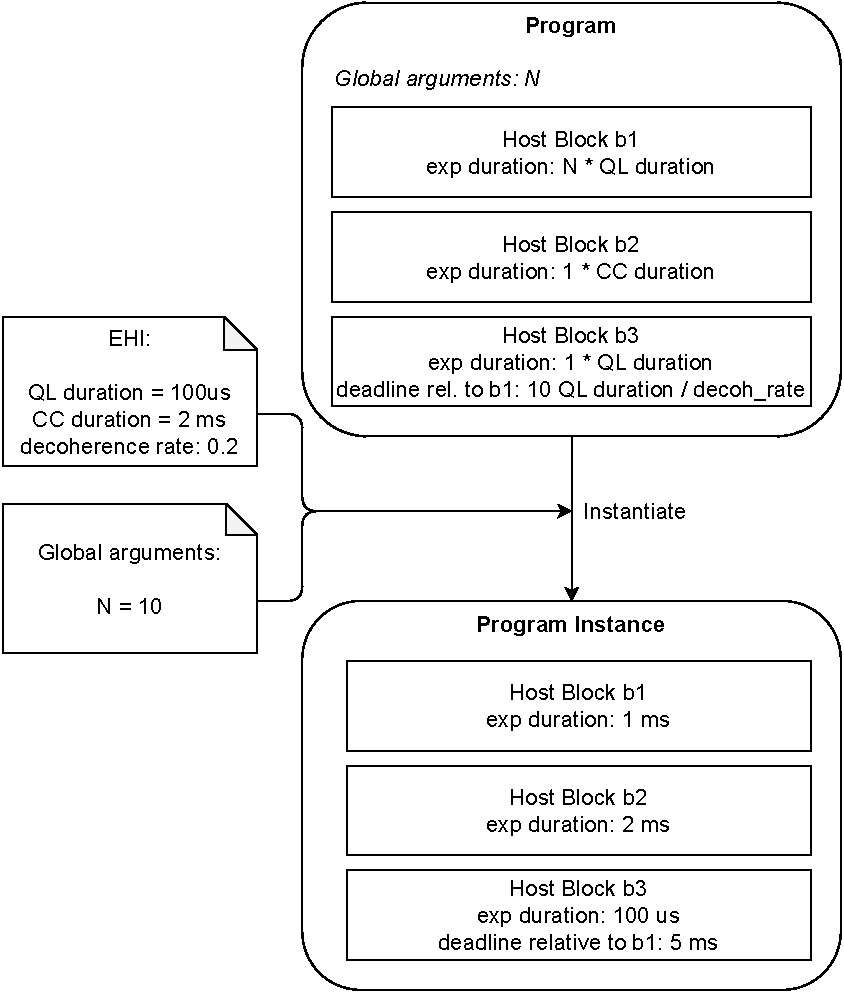
\includegraphics[width=0.6\textwidth]{figures/qoala/instantiation.pdf}
    \caption{Schematic example of program instantiation.
    A program containing global arguments ($N$) is instantiated using a concrete value for the arguments ($N = 10$) and the EHI (containing values for the expect duration of a QL block, the expected duration of a CC block, and the qubit noise parameter expressed as the \textit{decoherence rate}). This results in a program instance for which the expected durations have concrete values.
    }
    \label{qoala:fig:app:instantiation}
\end{figure}

\subsection{Program versus program instance}
A program is typically the output of a compiler.
For example, a compiler might produce a BQC-server program, including global arguments for the remote ID of the client (i.e. the client ID is \textit{not} hardcoded into it).
A program instance represents a single execution of a Qoala program with concrete values for its global arguments.
For instance, the client ID now has the explicit value of 3, since the remote client happens to have node ID 3.
Often many program instances may be created for a single program.
For example, if 1000 runs of the BQC program are desired, 1000 program instances are created based on the single Qoala program.

\paragraph{Batches}
A program may be submitted for execution in a batch.

A batch $B$ consists of a program $P$, the number of execution $N$ and inputs for each execution. Based on this, $N$ program instances are created.


\subsection{Shared memory}
\label{qoala:sec:app:shared_memory}
The CPS and QPS need to exchange information in order to execute local routines and request routines. They do so using shared memory.
The CPS writes routine arguments and reads results.
The QPS reads routine arguments and writes results.

Conflicts in writing and reading are avoided by the runtime itself (it is not assumed the hardware itself enforces read-only or write-only regions of memory).
This is achieved by strict read/write rules in Qoala: certain regions can only be written to by the CPS (QPS) while only be read from the QPS (CPS).
No region can be written to by both CPS and QPS.
Note that this design leaves open how the shared memory can be implemented: either as real physical shared memory, or as a message passing protocol.


\paragraph{Arrays}
The shared memory is logically divided into \textit{array elements} that can be allocated only by the CPS (\cref{qoala:fig:app:arrays}).
Each element can hold a single 32-bit signed integer.
The CPS can allocate shared memory space by specifying a \textit{size}, resulting in an allocated array.
An array is an ordered list of array elements. 
One can think of an array being a region in Shared Memory consisting of a consecutive list of elements.

Shared Memory is similar to the heap in classical OSes. Allocating an array is similar to \texttt{malloc} in C. Each program instance has its own view in the global shared memory, just like in classical OS, each program instance (or `process') has its own virtual memory space.

Elements that have been allocated but never written to have an undefined value.

An array may be named; it is written as \texttt{@arrayname}. An element in an array at index \texttt{i} is written as \texttt{@arrayname[i]}. This notation is used in NetQASM(\cref{qoala:sec:app:netqasm}).

Arrays are used to share data between the CPS and the QPS.
They are used for executing both LRs and RRs.

The shared memory is logically divided into 5 \textit{regions} (\cref{qoala:fig:app:shared_memory}).
Each of the regions contains array elements, and in each region, arrays can be allocated.
The regions are only a logical division, where each arrays in a certain region are only used to hold data for a specific use-case:

\begin{itemize}
\item \texttt{LR\_in}: Argument values for LRs. CPS writes, QPS reads.
\item \texttt{LR\_out}: Result values for LRs. CPS reads, QPS writes.
\item \texttt{RR\_in}: Argument values for RRs. CPS writes, QPS reads.
\item \texttt{RR\_ou}t: Result values for RRs. CPS reads, QPS writes.
\item \texttt{CR\_in}: Argument values for callback LRs. QPS reads, QPS writes.
\end{itemize}


\begin{figure}[t]
    \centering
    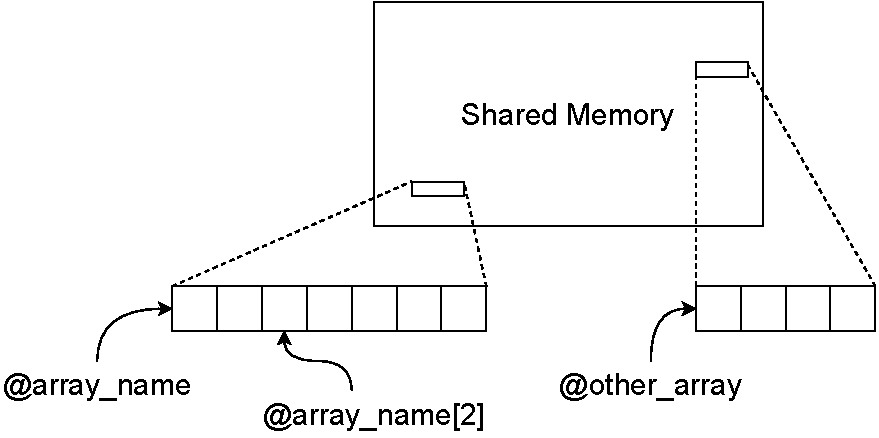
\includegraphics[width=0.6\textwidth]{figures/qoala/arrays.pdf}
    \caption{Schematic overview of shared memory, which is organized as \textit{arrays}.
    Arrays are allocated by the CPS with a certain size (the number of \textit{array elements}).
    Each array element holds a single classical value.
    Arrays are identified using the \texttt[@<name>] syntax.
    Particular array elements may be accessed using the \texttt{[index]} syntax.
    }
    \label{qoala:fig:app:arrays}
\end{figure}


\begin{figure}[t]
    \centering
    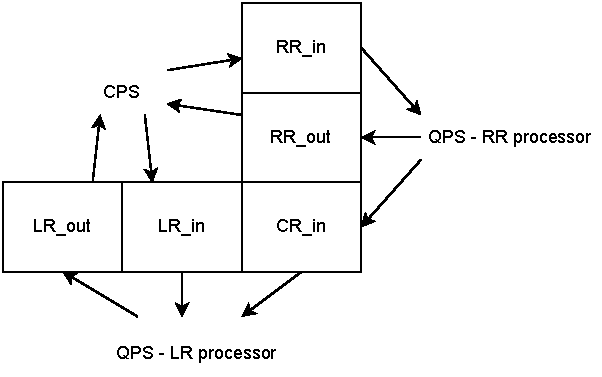
\includegraphics[width=0.6\textwidth]{figures/qoala/shared_memory.pdf}
    \caption{Shared memory regions.
    The CPS writes local routine arguments to the \texttt{LR\_in} section and request routine arguments to the \texttt{RR\_in} section.
    The CPS reads local routine results from the \texttt{LR\_out} section and request routine results from the \texttt{RR\_out} section.
    The QPS reads local routine arguments from \texttt{LR\_in} and write results to \texttt{LR\_out}.
    The QPS reads request routine arguments from \texttt{RR\_in} and write results to \texttt{RR\_out}.
    Callbacks for request routines use the separate \texttt{CR\_in} section to use request routine results as arguments of the callback local routine.
    }
    \label{qoala:fig:app:shared_memory}
\end{figure}


\paragraph{Arrays for local routines}
Before an local routine (LR) can be executed, two arrays must be allocated by the CPS:
\begin{itemize}
\item An array in the \texttt{LR\_in} region. Its size needs to match the number of arguments for the LR.
\item An array in the \texttt{LR\_out} region. Its size needs to match the number of results of the LR.
\end{itemize}

The array in the \texttt{LR\_in} region can be accessed by the NetQASM code in the LR body using the name \texttt{@input}.
The array in the \texttt{LR\_out} region can be accessed by the NetQASM code in the LR body using the name \texttt{@output}.

Note that each program instance allocates (at runtime) its own arrays. Each individual LR in each individual program instance has access to two arrays called \texttt{@input}  and \texttt{@output}, but in practice there can hence be multiple "input" and "output" arrays, each occupying a different part of the global Shared Memory.


\paragraph{Arrays for request routines}
Before a request routine (RR) can be executed, multiple arrays must be allocated by the CPS:
\begin{itemize}
\item An array in the \texttt{RR\_in} region. 
\item An array in the \texttt{RR\_out} region. Its size needs to match the number of names in the "Results" entry in the RR header.
\item An array in the \texttt{CR\_in} region. Its size needs to match the number of arguments for the callback LR of the RR.
\end{itemize}

The results of the RR are written to the array in the \mbox{\texttt{RR\_out}} region. Arguments to the callback LR are written to the array in the \texttt{CR\_in} region.



\subsection{Quantum memory}
\label{qoala:sec:app:quantum_memory}
The QPS is assumed to have access to a quantum random access memory (QRAM) consisting of \textit{qubits}.
Each qubit is a single location in the QRAM and can hold a single 2-dimensional quantum value, like $\ket{0}$ or $\ket{+}$.

We distinguish between (1) the \textit{physical quantum memory space (PQMS)} consisting of \textit{physical qubits}
and (2) a \textit{virtual quantum memory space (VQMS)} for each program instance (\cref{qoala:sec:runtime_environment}).

The topology (qubit connectivity) and noise characteristics of the PQMS are exposed as part of the EHI.
Each program instance has access to its own VQMS, which is represented as a Unit Module~\cite{dahlberg2022netqasm}.
The VQMS for each program instance is created when instantiating the program.
This can be seen as virtual memory allocation for the program.
At runtime, the VQMS of each running program instance is mapped to the PQMS.

\paragraph{Unit Modules}
A Unit Module (UM) describes the topology of a VQMS as well as its noise characteristics.
That is, a UM contains:
\begin{itemize}
\item \textbf{Qubit Info}: a list of all qubits available in the VQMS, with for each qubit the following information:
its virtual ID,
whether it is a communication qubit or not, and
its decoherence rate per second.

\item \textbf{Gate Info}: a list of all quantum gates and quantum local operations available for the qubits in the VQMS, with for each item the following information:
\begin{itemize}
  \item Which NetQASM instruction it is represented by (may be in a particular NetQASM flavor).
  \item On which sets of qubits the gate or operation can be applied.
  \item Its duration.
  \item The decoherence rate per second on each of the qubits it acts on.
\end{itemize}
\end{itemize}

A UM can be seen as a subset of the full EHI of a node, specifically containing a subset of all qubits available in the node.

Qubits in the Unit Module are called \textit{virtual qubits}. They are identified by their \textit{virtual IDs} and are mapped to physical qubits (\cref{qoala:fig:app:unit_module}).



\paragraph{Memory manager}
Quantum memory allocation and freeing is handled by a memory manager, which lives in the QPS.
The memory manager keeps track of the unit modules of all program instances, and maps virtual qubits to physical qubits. 

Before starting a local routine or request routine, the memory manager allocates the corresponding qubits.
For example, if a local routine for program instance $P$ defines in its metadata (see \cref{qoala:sec:app:program_structure}) that it uses virtual qubits 0 and 1, the memory manager allocates virtual qubits 0 and 1 (if not already allocated).
This involves finding currently unused physical qubits and mapping new virtual qubit to these free physical qubits.

\begin{figure}[t]
    \centering
    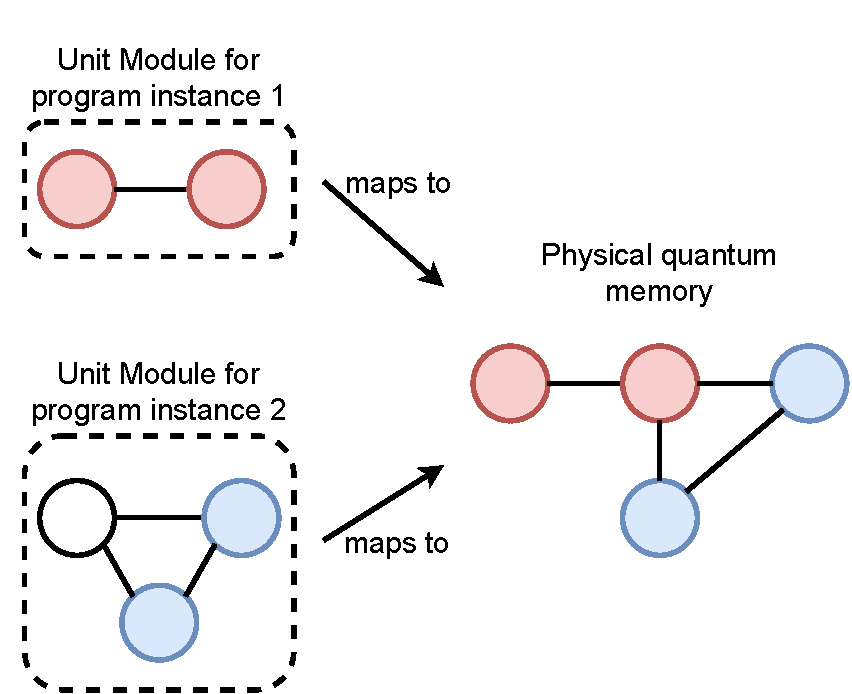
\includegraphics[width=0.6\textwidth]{figures/qoala/unit_module.pdf}
    \caption{Example of a physical quantum memory available in a node (four qubits) and two allocated unit modules. The colors of the qubits represent the physical locations they map to. Note that the top-left qubit of Unit Module 2 is not currently mapped and that it also cannot be mapped. Therefore, tasks that require program instance 2 to use a third qubit cannot be executed at this time.}
    \label{qoala:fig:app:unit_module}
\end{figure}



\subsection{Exposed hardware interface}
\label{qoala:sec:app:ehi}
The Qoala execution environment exposes certain information related to the hardware and software capabilities.
This information includes noise characteristics of quantum memory and of entanglement generation, as well as estimates of classical latencies.

All information that is exposed falls under the Exposed Hardware Interface (EHI).
The EHI can be divided into \textit{node info} and \textit{network info}.


\paragraph{EHI Node Info}
The EHI node info consists of:

\begin{itemize}
\item \textbf{Qubit Info}: a list of all qubits available at the node, with for each qubit the following information: 
(1) its ID,
(2) whether it is a communication qubit or not, and
(3) its decoherence rate per second.
\item \textbf{Gate Info}: a list of all quantum gates and quantum local operations available at the node, with for each item the following information:
(1) which NetQASM instruction it is represented by (may be in a particular NetQASM flavor,
(2) on which sets of qubits the gate or operation can be applied,
(3) its duration, and
(4) the decoherence rate per second on each of the qubits it acts on.

\item \textbf{NetQASM flavor}: a list of all supported NetQASM instructions. All NetQASM instructions mentioned in Gate Info must be in this list

\item \textbf{Classical latencies}:
Covers
(1) duration of executing a single QH Instruction, and
(2) duration of executing a classical NetQASM instruction (Note that the duration of quantum operations is covered by the Gate Info).
\end{itemize}

\paragraph{EHI Network Info}
The EHI network info consists of \textbf{Link Info} for each link in the network, with
(1) the expected duration of generating an entangled pair on this link, and
(2) the expected fidelity of generating an entangled pair on this link.



\subsection{Sockets}
Connections with remote nodes are modeled as \textit{sockets}.
Each program instance running on a node has access to classical sockets an EPR sockets.
Classical sockets represent an endpoint for connections over which classical messages can be sent.
A program instance can have classical sockets with any other nodes in the network.

An EPR socket represents an endpoint of a quantum connection.
Through the EPR socket, a program can ask for entanglement with a remote node.


\begin{sidewaysfigure}[t]
    \centering
    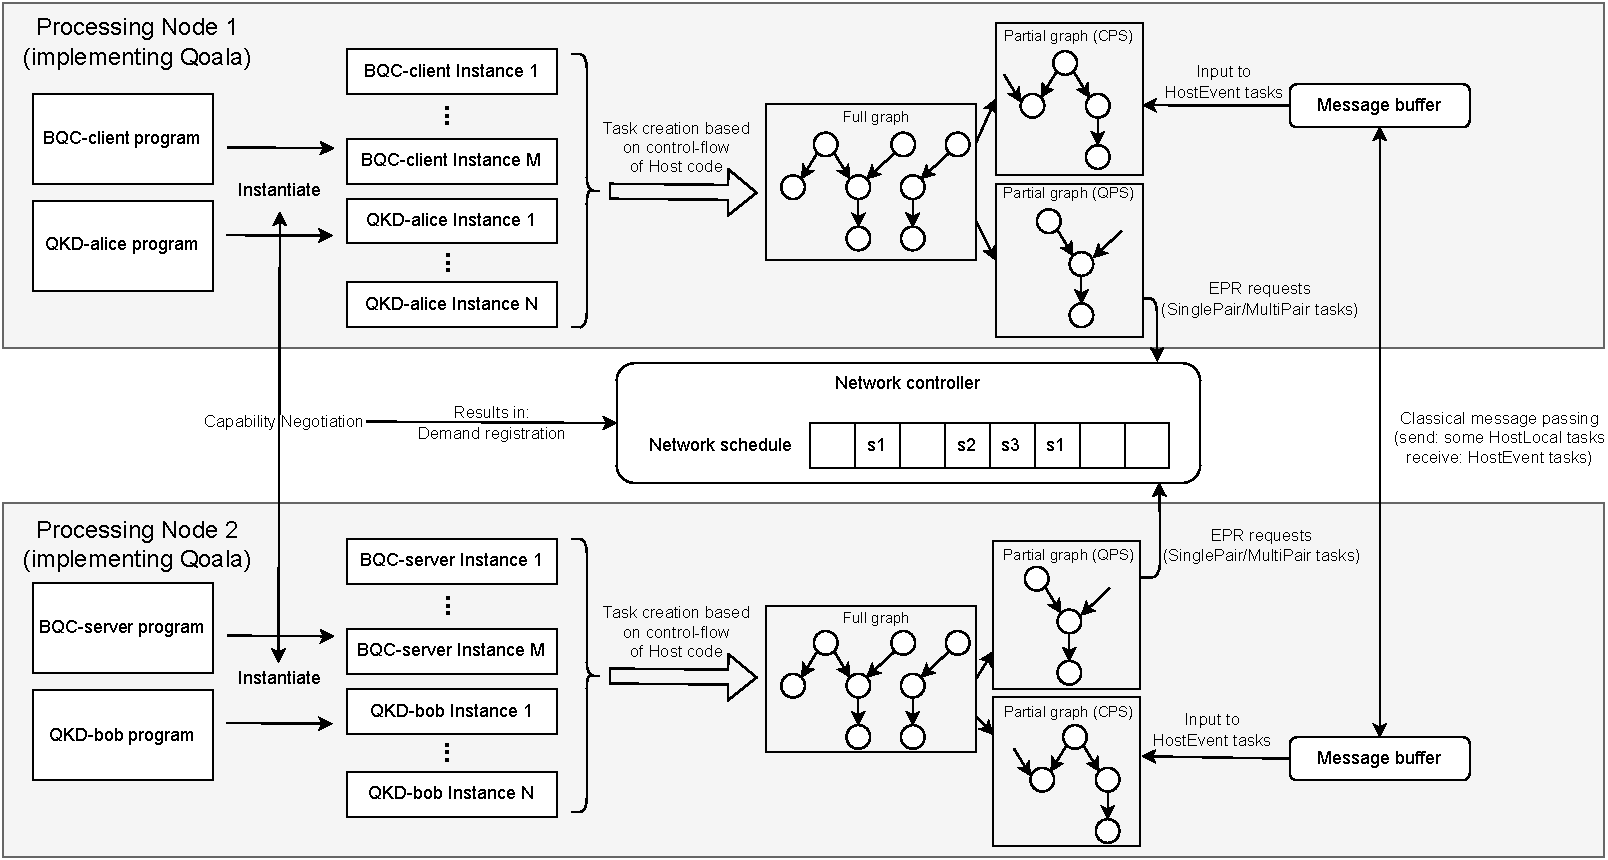
\includegraphics[width=\textwidth]{figures/qoala/runtime_detailed.pdf}
    \caption{Detailed Qoala runtime overview.}
    \label{qoala:fig:app:runtime_detailed}
\end{sidewaysfigure}

